\chapter{Introduction}
%St : 3

%Increasing resolution -> motivation and difficulties st 1
Throughout the history of astronomy, there have been celestial sources which appear point-like (unresolved) with the available instrumentation. To clarify the nature of these sources, ever more sophisticated instruments are developed. 

In principle, a diffraction-limited aperture can obtain an angular resolution of

\begin{equation}\label{eq:ang_res}
 \theta_{\rm res}\ \approx \ 1.22\ \lambda / D,
\end{equation}
where $D$ is the diameter of the aperture and $\lambda$ is the observing wavelength. However, dish apertures larger than a hundred metres are infeasible to construct while systematic errors, including scattering-induced blurring due to turbulence in the Earth's atmosphere can lead to instrument being unable to reach the diffraction limit. To overcome these difficulties and improve $\theta_{\rm res}$, a variety of new technologies have been developed, including space-based observatories which bypass the Earth's atmosphere, interferometric arrays which eliminate the need to build extremely large apertures, as well as mitigation strategies like adaptive optics and water vapour radiometry which account for atmospheric turbulence in real time.  


%Very Long Baseline Interferometry -> the highest resolution st 1
The astronomical observatory which typically achieves the highest angular resolution is Very Long Baseline Interferometry (VLBI). Interferometry  refers to the technique of measuring the electric field correlations between separated antennae pairs (referred to as `baselines'). The electric field correlations can be related to Fourier components on the sky and hence an approximate image of sky can be reconstructed through an `adequate' sampling of the Fourier domain and the inverse Fourier transform. With this method, the distance between the antennae effectively replaces $D$ in equation~\ref{eq:ang_res}, yielding far higher angular resolution than a single aperture. This technique is primarily used at radio frequencies as the phase of the electric field becomes unstable at shorter wavelengths, which causes the correlation to become incoherent. Hence, VLBI is simply radio interferometry with antennae separated by large distances, typically $\gtrsim 100$~km, including the possibility for antennae in Earth's orbit. The technique has seen several noteworthy achievements since its inception in the late 1960's, including resolution of the extra-galactic, compact, highly-variable objects, now known as quasars into core-jet systems, and the mapping of maser motion around the Supermassive Black Holes (SMBH) in the cores of nearby galaxies.

\section{The Event Horizon Telescope (EHT)}
% St: 3

% EHT -> intro to the Array st 1
In the last few decades there has been a push to enable VLBI capabilities at sub-millimetre wavelengths. This effort is being led by the Event Horizon Telescope consortium (EHT), an international project whose primary objective is to spatially resolve nearby black holes with an angular resolution on the order of their event horizons. In contrast to the previous state of the art high frequency VLBI observatory, the Very Long Baseline Array (VLBA) which has coverage to 87~GHz (3~mm), the EHT is currently observing at 230~GHz (1.3~mm) and will potentially extend till 315~GHz (0.8~mm) in the future. See Fig.~\ref{fig:eht_globe} for an annotated map of the locations of the EHT array. As the EHT will have baseline lengths comparable to the diameter of the earth, $|b| \sim 10^4$~km and is currently observing at 1.3~mm, this yields $\theta_{\rm res} \approx 30\ \mu$-arcsec.

%st 1
\begin{figure*}
\begin{center}
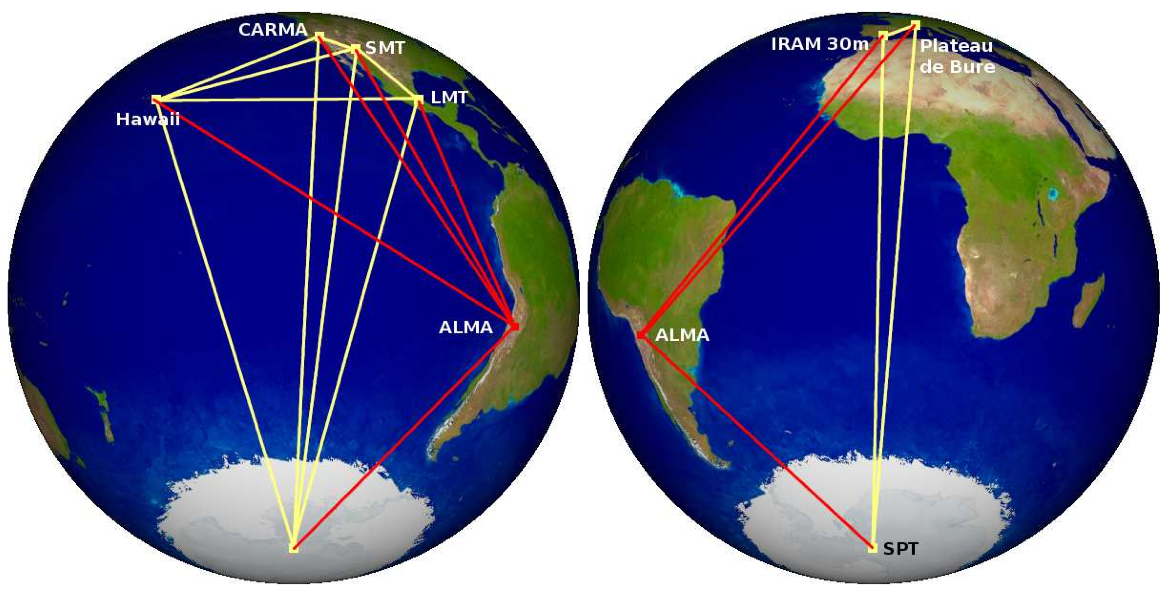
\includegraphics[width=0.8\columnwidth]{Images/eht_globe}
\caption{(Image credit: Remo Tilanius) The view of the Event Horizon Telescope (EHT) from Sgr~A*. This interferometric array uses Earth-diameter baselines, operating at $230-315$~GHz to attain resolution $\theta_{\rm res} \sim 10$ $\mu$-arcsec. Baselines to ALMA are shown in red, highlighting it's order of magnitude higher sensitivity. Note that the CARMA station has recently been discontinued, a telescope in Greenland is currently being constructed and there is ongoing investigation into a possible site in Southern Africa.\label{fig:eht_globe}%
}
\end{center}
\end{figure*}

% EHT -> intro to the science : scales 
To constrain the physics near a black hole, the observation needs to be sensitive to scales comparable to the event horizon. For a non-spinning (Schwarschild) black hole, the event horizon is spherically symmetric with a radius, 
\begin{equation}
R_{\rm Sch} = 2 G M_{\rm BH} /c^2,
\end{equation}
where $M_{\rm BH}$ is the black hole mass, $G$ is the gravitational constant and $c$ is the speed of light. The angular size of such an event horizon in the far field approximation is
\begin{align}
\theta_{\rm Sch} &= R_{\rm Sch} / d_{\rm src}\\
&\approx 0.02^{\prime \prime} \times 10^{-9} (M_{\rm BH}/M_\odot)({\rm kpc}/d_{\rm src}),
\end{align}
where $d_{\rm src}$ is the distance from observer to source. For Sgr~A$^\star$ and M87 [refs..], this results in $\theta_{\rm Sch} \sim 5-10\ \mu$-arcsec.

%Lensing and the photon ring 
Fortunately, the innermost emission is gravitationally lensed by the SMBH, which causes it to appear magnified by several times its original size. In theory, the innermost orbit should be inhabited by a ring of photons, the lensed image of which should produce a shadow-like (or `silhouette') feature \citep{Doeleman_2010}. Fig.~\ref{fig:grmhd} shows an image ray-traced from a General Relativistic Magneto-Hydrodyanmic simulation of the accretion disc around Sgr~A* \citep{Moscibrodzka_2014}, with the dark silhouette clearly shown in the centre. The two primary targets Sgr~A$^\star$ and M87 are expected to have gravitationally-lensed photon rings with apparent angular diameters of $\theta_{\rm pr} \sim 50$ and $\sim 20-40\ \mu$-arcsec respectively \citep*{Falcke_2013,Broderick_2009}, and should be resolvable by the EHT. Note that the large range for M87 is due to the current controversy between stellar and dust traces of its mass.
% Emission and optical depth
There are two other important reasons why this observation needs to be conducted at sub-millimetre frequencies, as opposed to a longer wavelength orbiting VLBI observation which is possible with the RadioAstron space observatory. Firstly as the power spectrum of Sgr~A$^\star$ peaks in sub-millimetre \citep{Serabyn_1997,Falcke_1998}

it is important for observing the innermost emission is that it must be optically thin. As the power spectrum of Sgr~A$^\star$ peaks in sub-millimetre \citep{Serabyn_1997,Falcke_1998}.The interferometric technique also works to filter out the smooth emission. 

%ISM blurring
The extreme angular resolution required, blurring effects due to scattering by the interstellar medium \citep[ISM; e.g.][]{Fish_2014} necessitate that the EHT be comprised of antennas separated by at least thousands of kilometres that operate at high radio frequency ($\nu>200$~GHz).  

\begin{figure*}
\begin{center}
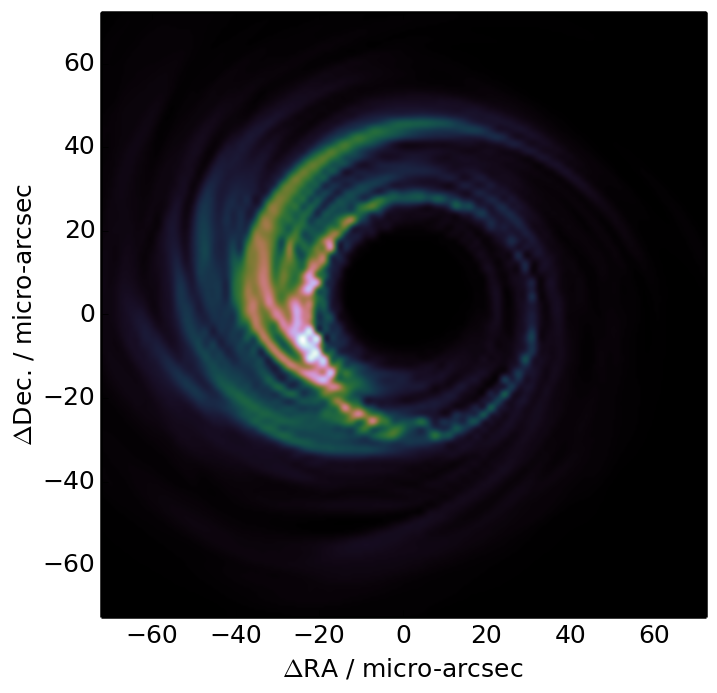
\includegraphics[width=0.5\columnwidth]{Images/disk30}
\caption{(Image credit: Monika Moscibrodzka) GR-MHD simulation of an accretion disk inclined at $30^\circ$ around Sgr~A* \citep{Moscibrodzka_2014}. Note the dark area in the centre, known as the black hole shadow which represents the lensed image of the photon ring orbiting the BH. A measurement of it's precise shape is a test of general relativity in the strong field regime. Note that the asymmetry in the image is due to doppler boosting, and we are seeing all sides of the disk through lensing. \label{fig:grmhd}%
}
\end{center}

\end{figure*}


%Probing strong gravity and black hole spacetime St 3
Gravity as described by General Relativity (GR) is consistent with all observational experiments, however GR has conceptual weaknesses, especially as it is not compatible with the quantum description of reality \citep{Goddi_2016}. Various alternatives to GR have been theorised which do not assume a purely classical description of matter. To test GR against it's numerous alternatives, we have to observe gravity in the regime where we expect the largest observational deviations a GR prediction would have if it were only an approximate theory of gravity. The space-time close to a SMBH is an ideal candidate, as the gravitational effects are very strong. Lensed emission of the gravitational lensed photon ring.  The exact sizes and shapes of which indicate different spacetime and theories of gravity. Note that even in this regime, the deviation from GR is small. We can also explore black hole physics by testing the no-hair theorem or that black holes are only described by their mass, spin and charge by constraining the quadrapole moment of the black hole.deviations
from the Kerr metric

{\bf FIG. Plot of analytic shapes and sizes of the bh shadow from the predictions of different theories of gravity}\\
~\\


%Probing  AGN accretion and jet launch astrophysics
%Pr : 3,St: 3
{\bf [AGN jet basics.]}

Astrophysical jets were first discovered over a century ago, accretion onto a black hole was first postulated to power these jet by .. .However a century later, the mechanism of accretion and jet launching ifrom SMBH are still highly debated. 

\textbf{Fig: Typical AGN jet illustration showing magnetic fields }

Recently an industry of sophiscated General Relativistic Magneto-Hydrodyanmic (GRMHD) simulations has developed yielding important insights but also new questions. Now, mm-VLBI has the opportunity of constrains the mechanisms. Specifically we can map the magnetic field configuration, which is a key aspect using polarimetry and Faraday Rotation. The quiescent and variability structure and also be explore in total intensity. Flaring structure.  Distiniguish between accretion disk and inner jet. Distinguish between the different Jet and Disk models for each bh. Deterimine spin.\\
~\\
\textbf{Fig: 2/3 panels of simulated images of disk and jet models of Sgr A*/M87}\\

In M87, where the jet is dominant, micro-arcsecond scale astrometry, capable with the EHT, can determine the distance from the jet base from the event horizon, as well as the width of the jet base. Opening up new possibilities in explore particle production and other exotic physics occuring at the event horizon. 


\textbf{Fig: 2/3 panels of simulated polarimetric images of Sgr A*/M87 showing ordered magnetic fields}

\subsection{Challenges and obstacles}
%Pr : 2, St : 2
%Overview of challenges
Performing Very Long Baseline Interometry (VLBI) at mm-wavelengths presents unique calibration challenges, including very short atmospheric coherence times that are typically $\lesssim$10~s \citep{Doeleman_2009}, low calibrator source sky density, complex and variable calibrator source structure, and antenna pointing accuracies that are a non-negligible fraction of the antenna primary beam. Addition These effects may place significant limitations on the sensitivity, image fidelity, and dynamic range that can be achieved with mm-VLBI.  Performing mm-VLBI however, is a difficult task for a variety of reasons. Firstly the arrays are inhomogenous, made up of a collections of different stations working together, Difficult to get time on all the stations. there are a variety of signal corruptions which take place. Briefly introduce signal corruptions, variability, ..etc, how these represent calibration and interpretation challenges.


% Effect of corruptions on Science extraction : parameter estimation and imaging, %High accuracy needed for science 
%Pr : 2, St : 3

we need to measure the fractional
asymmetry of the shadow shape with respect to its angular size to the few percent


~Estimating the `macro'-parameters of Sgr A*, spin, orientation, position angle through a Bayesian parameter estimation analysis with closure quantities\\
Furthermore, unaccounted for systematic and/or non-Gaussian uncertainties could preclude robust, accurate Bayesian parameter estimation and model selection analyses of accretion flow \citep[e.g.][]{Broderick_2016} and gravitational physics \citep[e.g.][]{Broderick_2014, Psaltis_2016}, two of the EHT's many objectives.
~\\
see psaltis 2015 for  some other shadow detection criteria
\textbf{Fig: A Broderick 2016 posterior probability distribution (?)}


\section{A realistic mm-VLBI simulator}
%Pr : 1 : St : 1

%Why simulate: intro
Given the significant observation challenges that the EHT faces, we have undertaken this project to build a mm-VLBI observation and signal corruption simulator.  There are many benefits for using such a toolkit and indeed synthetic data simulation is common practice for every major scientific experiment. Two prominent examples is the  extensive synthetic data generation for gravitational wave template matching for LIGO (ref) or for LHC particle collision experiments (ref). In essence such a simulator would fill in the final part of the theoretical signal propagation chain, effectively taking  astrophysical simulations of the source (e.g. SMBH) as an input and returning realistic synthetic data. This allows a more effective interplay between theory and observation. The remainder of this section will briefly discuss several use cases for an EHT synthetic data simulator and how we have designed the software to meet these requirements. 

%Specific use cases of simulations

%Testing calim through standard challenges
A key observational use case is the testing of calibration, parameter estimation and imaging algorithms and strategies. As the inputs to the simulator are known exactly, when passing simulated data through the data processing pipelines, we are better able to explore sources of error which are difficult to disentangle from intrinsic source features in real data.  A straightforward way to perform such a test is through the creation of a set of `standard challenge' dataset. Such datasets would be available to the entire community input into their calibration and/or imaging routines. Following this, a detailed comparison between the different strategies in varying regimes (source and other factors) can be made. Importantly, a systematic investigation of a particular algorithm across many different datasets could provide insight into subtle or previously unknown sources of error.

%bayesian parameter estimation
Bayesian parameter estimation and model selection analyses of accretion flow \citep[e.g.][]{Broderick_2016} and gravitational physics \citep[e.g.][]{Broderick_2014, Psaltis_2016} offer a promising approach to constrain theoretical models when using visibilities or visibility derived quantities. However, unaccounted systematic errors in the signal processing chain could bias  the posterior probability distribution, precluding a robust and accurate determination of key science parameters. Through the construction of an end-to-end simulation pipeline, the Bayesian parameter estimation procedure extended to handle more realistic synthetic data. This would entail combining many iterations data simulator with a solver to perform calibration and parameter estimation. %leave for now

%Optimising observations
Simulated data can also assist in the optimisation of the experimental configuration. Financial constrains require the prioritisation of hardware upgrades e.g. increasing bandwidth, surface accuracy improvement, deployment of water vapour radiometers or additional receiver bands. Simulated data together with calibration and imaging pipelines can help to quantify the benefit of each improvement based on expected scientific return. This approach can even be extended to assess new candidate stations, especially as new geographic locations e.g. in Southern Africa are receiving increasing attention due to the potential long baselines to ALMA, SPT and European stations.

%other simulation efforts
Recently, there has been an increase in the attention given to simulating EHT observations of Sgr~A$^*$ (\citealt{Fish_2014}; \citealt{Lu_2014}; \citealt{2015arXiv151201413B}). However, these are primarily focused on image reconstruction and assume perfect phase calibration i.e. no troposphere-induced fringe-fitting errors; perfect antenna pointing accuracy; perfect phasing efficiency; and in most cases simple, non-variable Gaussian kernel smoothing to simulate ISM scattering. Clearly, as the EHT array is enhanced (and likely expanded), so too must the interferometric simulations evolve to provide ever-more realistic predictions on the confidence levels with which parameters can be extracted and hence exclude theoretical models of gravity and/or accretion flows.

%the Meqtrees+MS approach

Over the past decade, significant effort has been placed on advanced radio interferometric calibration and imaging algorithms for centimetre and metre-wave facilities in response to the large number of new arrays in construction or design phase (e.g. MeerKAT, ASKAP, SKA, LOFAR, HERA). A leading software package in this pursuit is \textsc{MeqTrees}\footnote{https://ska-sa.github.io/meqtrees/} \citep*{Noordam_2010}, which was developed to simulate, understand and address the calibration issues to be faced with the greatly enhanced sensitivity, instantaneous bandwidth, and field-of-view of such facilities. For example, \textsc{MeqTrees} is rooted in the Measurement Equation mathematical formalism \citep{Hamaker_1996}, which parameterizes the signal path into distinct $2 \times 2$ complex  matrices called Jones matrices. This formalism and applications thereof are laid out in \citep{Smirnov_2011a,Smirnov_2011b,Smirnov_2011c} and are arbitrarily generalized to model any (linear) effect, including undesired signal corruptions that often may have subtle yet systematic effects. \textsc{MeqTrees} has been applied to correct for direction dependent calibration errors to JVLA and WSRT observations, achieving record-breaking high dynamic range images \citep{Smirnov_2011c}. The effectiveness provided by the Measurement Equation formalism in radio interferometric calibration provides a strong motivation to explore its application to challenging goal of imaging a supermassive black hole silhouette with mm-VLBI. To construct this simulator we leverage off metre and cm-wavelength simulation and calibration successes and build a \textsc{MeqTrees}-based mm-VLBI-specific software package which we name, \textsc{MeqSilhouette}.  Use of \textsc{MeqTrees} and \textsc{measurement set} data format lends itself to investigating a range of different techniques that are used in other areas of interferometry (e.g. coh-Jones paper). While \textsc{MeqTrees} has not yet been used in the context of mm-wavelength observations, the framework is agnostic to higher frequency implementation as long as the Measurement Equation is appropriately constructed. This technology enables us to


\section{Outline}



















